%\documentclass[dvipdfmx,autodetect-engine,10pt,b5paper,papersize,openany]{jsbook}
\documentclass[dvipdfmx,autodetect-engine,10pt,b5paper,papersize,openany,dvipsnames]{jsbook}

\usepackage{color}
\usepackage{titlesec}
\usepackage{multicol}

% https://tex.stackexchange.com/questions/12262/multicol-and-figures
%\newenvironment{Figure}
%  {\par\medskip\noindent\minipage{\linewidth}}
%  {\endminipage\par\medskip}

% https://puarts.com/?pid=1014
\makeatletter
\newenvironment{Figure}
  {\def\@captype{figure}}
  {}
\makeatother

\usepackage{amsmath,txfonts}
\usepackage{bm}
\usepackage{mathrsfs} % \mathscr
\usepackage[dvipdfmx]{graphicx}

\usepackage{tikzpagenodes}


%\usepackage{xcolor}
\usepackage[object=vectorian]{pgfornament}
\usetikzlibrary{shapes.geometric,calc}

\usepackage{calligra}
\usepackage[T1]{fontenc}


%\usepackage[dvipdfmx]{hyperref}
\usepackage[hidelinks]{hyperref}
\usepackage{pxjahyper}

% https://oku.edu.mie-u.ac.jp/~okumura/jsclasses/
% jsbook の余白が広すぎます
% 書籍では1行の長さが全角40文字を超えないようにしています。
% そのため,段組をしないときは,自動的にどちらかの余白が広くなります
% (美文書シリーズのようなデザインになります)。
% これが困るときはプリアンブル(\begin{document} の前)に次のように書いてください。
\setlength{\textwidth}{\fullwidth}
\setlength{\evensidemargin}{\oddsidemargin}


\begin{document}


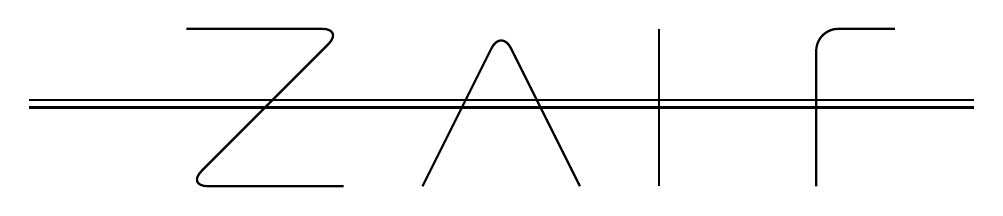
\begin{tikzpicture}
  \draw[thick,rounded corners=8pt]
    (2, 2) -- (4, 2) -- (2, 0) -- (4, 0);
  \draw[thick,rounded corners=8pt]
    (5, 0) -- (6, 2) -- (7, 0);
  \draw[thick,rounded corners=8pt]
    (8, 0) -- (8, 2);
  \draw[thick,rounded corners=8pt]
    (10, 0) -- (10, 2) -- (11, 2);
  \draw[thick,rounded corners=8pt]
    (0, 1) -- (12, 1);
  \draw[thick,rounded corners=8pt]
    (0, 1.1) -- (12, 1.1);
\end{tikzpicture}

\vspace{2cm}

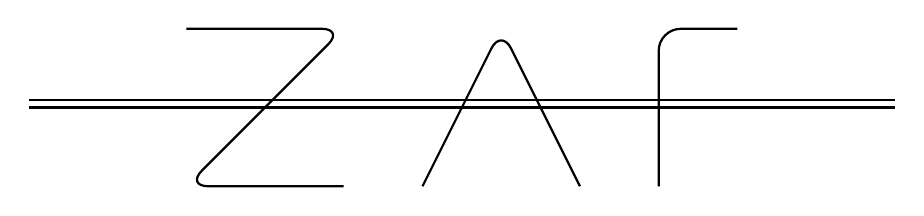
\begin{tikzpicture}
  \draw[thick,rounded corners=8pt]
    (2, 2) -- (4, 2) -- (2, 0) -- (4, 0);
  \draw[thick,rounded corners=8pt]
    (5, 0) -- (6, 2) -- (7, 0);
  \draw[thick,rounded corners=8pt]
    (8, 0) -- (8, 2) -- (9, 2);
  \draw[thick,rounded corners=8pt]
    (0, 1) -- (11, 1);
  \draw[thick,rounded corners=8pt]
    (0, 1.1) -- (11, 1.1);
\end{tikzpicture}

\vspace{2cm}

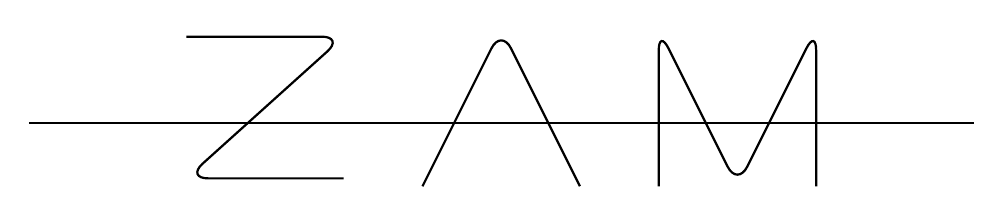
\begin{tikzpicture}
  \draw[thick,rounded corners=8pt]
    (2, 1.9) -- (4, 1.9) -- (2, 0.1) -- (4, 0.1);
  \draw[thick,rounded corners=8pt]
    (5, 0) -- (6, 2) -- (7, 0);
  \draw[thick,rounded corners=8pt]
    (8, 0) -- (8, 2) -- (9, 0) -- (10, 2) -- (10, 0);
  \draw[thick,rounded corners=8pt]
    (0, 0.8) -- (12, 0.8);
\end{tikzpicture}

\vspace{2cm}

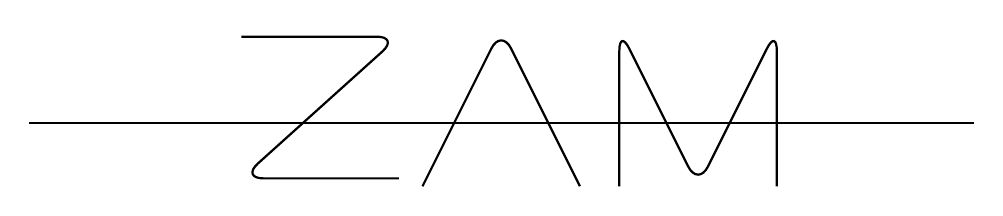
\begin{tikzpicture}
  \draw[thick,rounded corners=8pt]
    (2.7, 1.9) -- (4.7, 1.9) -- (2.7, 0.1) -- (4.7, 0.1);
  \draw[thick,rounded corners=8pt]
    (5, 0) -- (6, 2) -- (7, 0);
  \draw[thick,rounded corners=8pt]
    (7.5, 0) -- (7.5, 2) -- (8.5, 0) -- (9.5, 2) -- (9.5, 0);
  \draw[thick,rounded corners=8pt]
    (0, 0.8) -- (12, 0.8);
\end{tikzpicture}

\vspace{2cm}

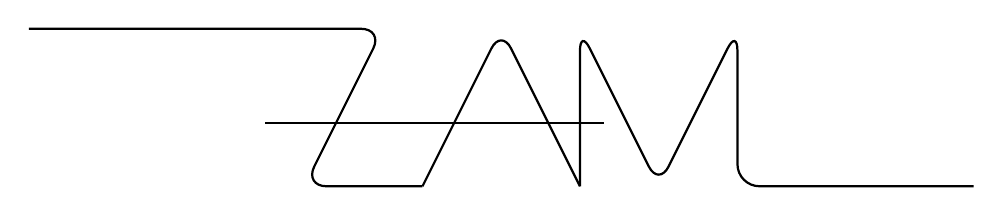
\begin{tikzpicture}
  \draw[thick,rounded corners=8pt]
    (0, 2) -- (4.5, 2) -- (3.5, 0) -- (5, 0);
  \draw[thick,rounded corners=8pt]
    (5, 0) -- (6, 2) -- (7, 0);
  \draw[thick,rounded corners=8pt]
    (7, 0) -- (7, 2) -- (8, 0) -- (9, 2) -- (9, 0) -- (12, 0);
  \draw[thick,rounded corners=8pt]
    (3, 0.8) -- (7.3, 0.8);
\end{tikzpicture}

\newpage

\vspace{2cm}

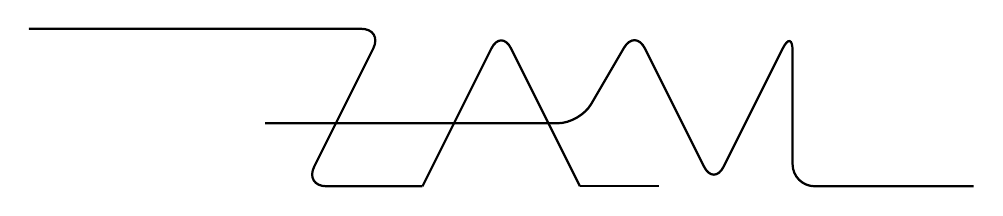
\begin{tikzpicture}
  \draw[thick,rounded corners=8pt]
    (0, 2) -- (4.5, 2) -- (3.5, 0) -- (5, 0);
  \draw[thick,rounded corners=8pt]
    (5, 0) -- (6, 2) -- (7, 0);
  \draw[thick,rounded corners=8pt]
    (7, 0) -- (8, 0);
  \draw[thick,rounded corners=8pt]
    (3, 0.8) -- (7, 0.8)
    -- (7.7, 2) -- (8.7, 0) -- (9.7, 2) -- (9.7, 0) -- (12, 0);
\end{tikzpicture}

\vspace{2cm}

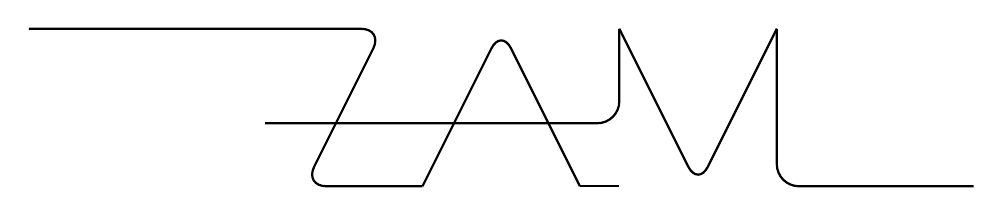
\begin{tikzpicture}
  \draw[thick,rounded corners=8pt]
    (0, 2) -- (4.5, 2) -- (3.5, 0) -- (5, 0);
  \draw[thick,rounded corners=8pt]
    (5, 0) -- (6, 2) -- (7, 0);
  \draw[thick,rounded corners=8pt]
    (7, 0) -- (7.5, 0);
  \draw[thick,rounded corners=8pt]
    (3, 0.8) -- (7.5, 0.8) -- (7.5, 2);
  \draw[thick,rounded corners=8pt]
    (7.5, 2)  -- (8.5, 0) -- (9.5, 2);
  \draw[thick,rounded corners=8pt]
    (9.5, 2) -- (9.5, 0) -- (12, 0);
\end{tikzpicture}

\vspace{2cm}

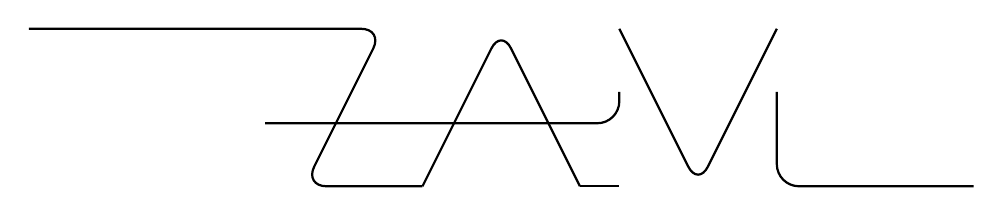
\begin{tikzpicture}
  \draw[thick,rounded corners=8pt]
    (0, 2) -- (4.5, 2) -- (3.5, 0) -- (5, 0);
  \draw[thick,rounded corners=8pt]
    (5, 0) -- (6, 2) -- (7, 0);
  \draw[thick,rounded corners=8pt]
    (7, 0) -- (7.5, 0);
  \draw[thick,rounded corners=8pt]
    (3, 0.8) -- (7.5, 0.8) -- (7.5, 1.2);
  \draw[thick,rounded corners=8pt]
    (7.5, 2)  -- (8.5, 0) -- (9.5, 2);
  \draw[thick,rounded corners=8pt]
    (9.5, 1.2) -- (9.5, 0) -- (12, 0);
\end{tikzpicture}

\newpage

\section{アニメーション的に}

% 0
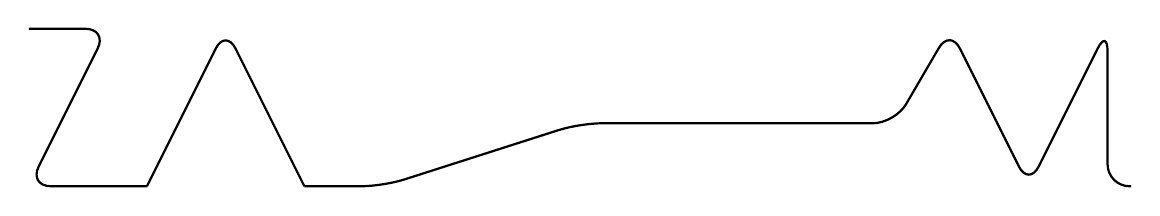
\begin{tikzpicture}
  \begin{scope}[thick,rounded corners=8pt]
  \draw (0, 2) -- (1, 2) -- (0, 0) -- (1.5, 0);
  \draw (1.5, 0) -- (2.5, 2) -- (3.5, 0);
  \draw (3.5, 0) -- (4.5, 0)
    -- (7, 0.8) -- (11, 0.8)
    -- (11.7, 2) -- (12.7, 0) -- (13.7, 2) -- (13.7, 0) -- (14, 0);
  \end{scope}
\end{tikzpicture}

\vspace{1cm}

% 1
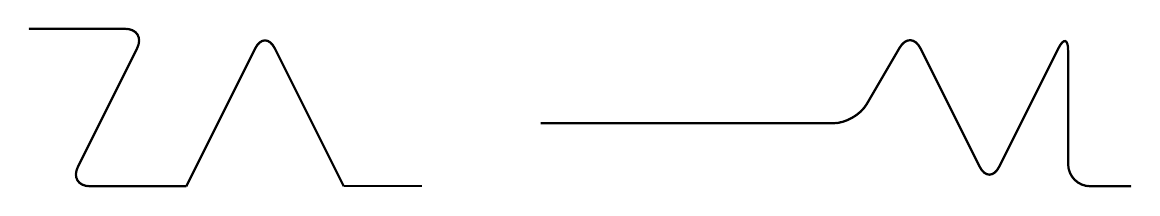
\begin{tikzpicture}
  \begin{scope}[thick,rounded corners=8pt]
  \draw (0, 2) -- (1.5, 2) -- (0.5, 0) -- (2, 0);
  \draw (2, 0) -- (3, 2) -- (4, 0);
  \draw (4, 0) -- (5, 0);
  \draw (6.5, 0.8) -- (10.5, 0.8)
    -- (11.2, 2) -- (12.2, 0) -- (13.2, 2) -- (13.2, 0) -- (14, 0);
  \end{scope}
\end{tikzpicture}

\vspace{1cm}

% 2
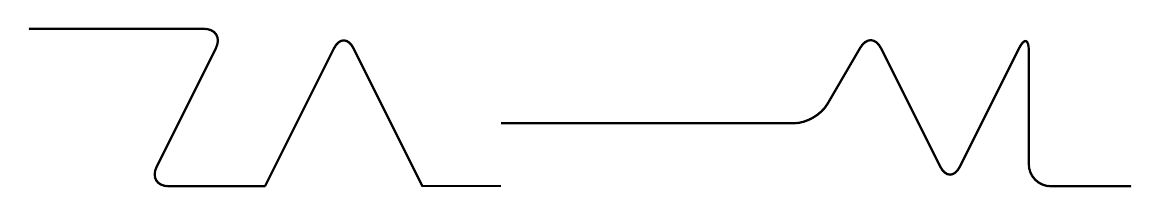
\begin{tikzpicture}
  \begin{scope}[thick,rounded corners=8pt]
  \draw (0, 2) -- (2.5, 2) -- (1.5, 0) -- (3, 0);
  \draw (3, 0) -- (4, 2) -- (5, 0);
  \draw (5, 0) -- (6, 0);
  \draw (6, 0.8) -- (10, 0.8)
    -- (10.7, 2) -- (11.7, 0) -- (12.7, 2) -- (12.7, 0) -- (14, 0);
  \end{scope}
\end{tikzpicture}

\vspace{1cm}

% 3
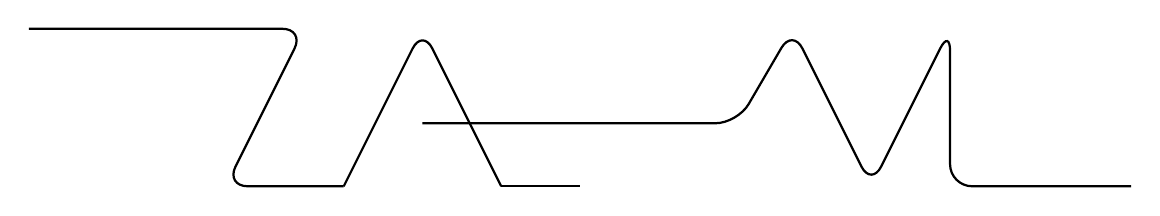
\begin{tikzpicture}
  \begin{scope}[thick,rounded corners=8pt]
  \draw (0, 2) -- (3.5, 2) -- (2.5, 0) -- (4, 0);
  \draw (4, 0) -- (5, 2) -- (6, 0);
  \draw (6, 0) -- (7, 0);
  \draw (5, 0.8) -- (9, 0.8)
    -- (9.7, 2) -- (10.7, 0) -- (11.7, 2) -- (11.7, 0) -- (14, 0);
  \end{scope}
\end{tikzpicture}

\vspace{1cm}

% 4
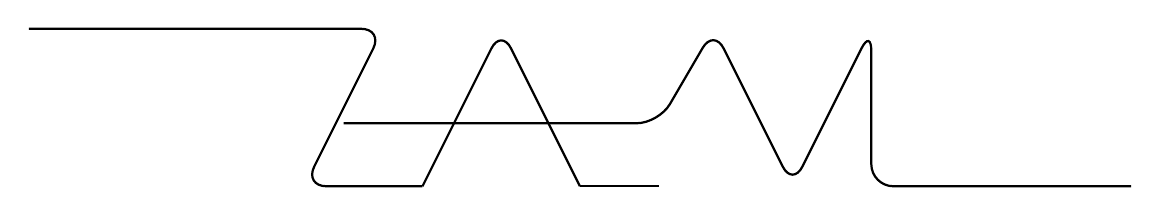
\begin{tikzpicture}
  \begin{scope}[thick,rounded corners=8pt]
  \draw (0, 2) -- (4.5, 2) -- (3.5, 0) -- (5, 0);
  \draw (5, 0) -- (6, 2) -- (7, 0);
  \draw (7, 0) -- (8, 0);
  \draw (4, 0.8) -- (8, 0.8)
    -- (8.7, 2) -- (9.7, 0) -- (10.7, 2) -- (10.7, 0) -- (14, 0);
  \end{scope}
\end{tikzpicture}

\vspace{1cm}

% 5
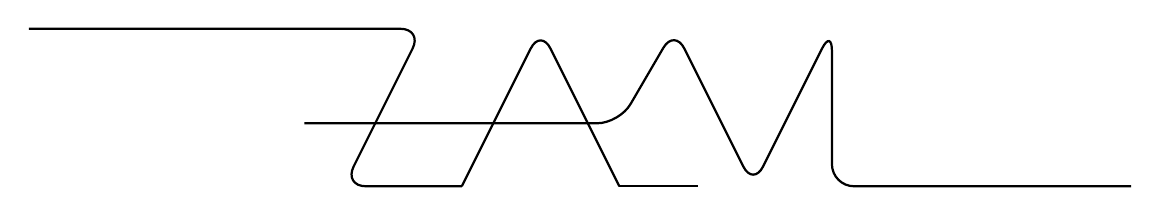
\begin{tikzpicture}
  \begin{scope}[thick,rounded corners=8pt]
  \draw (0, 2) -- (5, 2) -- (4, 0) -- (5.5, 0);
  \draw (5.5, 0) -- (6.5, 2) -- (7.5, 0);
  \draw (7.5, 0) -- (8.5, 0);
  \draw (3.5, 0.8) -- (7.5, 0.8)
    -- (8.2, 2) -- (9.2, 0) -- (10.2, 2) -- (10.2, 0) -- (14, 0);
  \end{scope}
\end{tikzpicture}



\newpage

\section{重ねる}

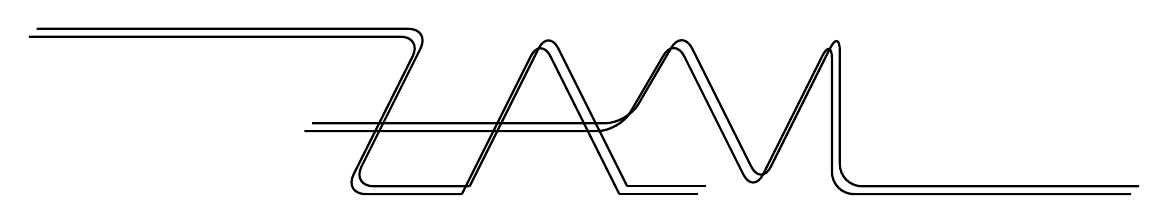
\begin{tikzpicture}
  \draw[thick,rounded corners=8pt]
    (0, 2) -- (5, 2) -- (4, 0) -- (5.5, 0);
  \draw[thick,rounded corners=8pt]
    (5.5, 0) -- (6.5, 2) -- (7.5, 0);
  \draw[thick,rounded corners=8pt]
    (7.5, 0) -- (8.5, 0);
  \draw[thick,rounded corners=8pt]
    (3.5, 0.8) -- (7.5, 0.8)
    -- (8.2, 2) -- (9.2, 0) -- (10.2, 2) -- (10.2, 0) -- (14, 0);

  \begin{scope}[xshift=0.1cm,yshift=0.1cm]
  \draw[thick,rounded corners=8pt]
    (0, 2) -- (5, 2) -- (4, 0) -- (5.5, 0);
  \draw[thick,rounded corners=8pt]
    (5.5, 0) -- (6.5, 2) -- (7.5, 0);
  \draw[thick,rounded corners=8pt]
    (7.5, 0) -- (8.5, 0);
  \draw[thick,rounded corners=8pt]
    (3.5, 0.8) -- (7.5, 0.8)
    -- (8.2, 2) -- (9.2, 0) -- (10.2, 2) -- (10.2, 0) -- (14, 0);
  \end{scope}[yshift=0.1cm]
\end{tikzpicture}


\begin{tikzpicture}
  \begin{scope}[thick, rounded corners=8pt,color=red]
  \draw (0, 2) -- (5, 2) -- (4, 0) -- (5.5, 0);
  \draw (5.5, 0) -- (6.5, 2) -- (7.5, 0);
  \draw (7.5, 0) -- (8.5, 0);
  \draw (3.5, 0.8) -- (7.5, 0.8)
    -- (8.2, 2) -- (9.2, 0) -- (10.2, 2) -- (10.2, 0) -- (14, 0);
  \end{scope}

  \begin{scope}[thick, rounded corners=8pt,color=orange,
      xshift=0.04cm,yshift=-0.1cm]
  \draw (0, 2) -- (5, 2) -- (4, 0) -- (5.5, 0);
  \draw (5.5, 0) -- (6.5, 2) -- (7.5, 0);
  \draw (7.5, 0) -- (8.5, 0);
  \draw (3.5, 0.8) -- (7.5, 0.8)
    -- (8.2, 2) -- (9.2, 0) -- (10.2, 2) -- (10.2, 0) -- (14, 0);
  \end{scope}

  \begin{scope}[thick, rounded corners=8pt,color=yellow,
      xshift=0.08cm,yshift=-0.2cm]
  \draw (0, 2) -- (5, 2) -- (4, 0) -- (5.5, 0);
  \draw (5.5, 0) -- (6.5, 2) -- (7.5, 0);
  \draw (7.5, 0) -- (8.5, 0);
  \draw (3.5, 0.8) -- (7.5, 0.8)
    -- (8.2, 2) -- (9.2, 0) -- (10.2, 2) -- (10.2, 0) -- (14, 0);
  \end{scope}

  \begin{scope}[thick, rounded corners=8pt,color=green,
      xshift=0.12cm,yshift=-0.3cm]
  \draw (0, 2) -- (5, 2) -- (4, 0) -- (5.5, 0);
  \draw (5.5, 0) -- (6.5, 2) -- (7.5, 0);
  \draw (7.5, 0) -- (8.5, 0);
  \draw (3.5, 0.8) -- (7.5, 0.8)
    -- (8.2, 2) -- (9.2, 0) -- (10.2, 2) -- (10.2, 0) -- (14, 0);
  \end{scope}

  \begin{scope}[thick, rounded corners=8pt,color=blue,
      xshift=0.16cm,yshift=-0.4cm]
  \draw (0, 2) -- (5, 2) -- (4, 0) -- (5.5, 0);
  \draw (5.5, 0) -- (6.5, 2) -- (7.5, 0);
  \draw (7.5, 0) -- (8.5, 0);
  \draw (3.5, 0.8) -- (7.5, 0.8)
    -- (8.2, 2) -- (9.2, 0) -- (10.2, 2) -- (10.2, 0) -- (14, 0);
  \end{scope}

  \begin{scope}[thick, rounded corners=8pt,color=BlueViolet,
      xshift=0.2cm,yshift=-0.5cm]
  \draw (0, 2) -- (5, 2) -- (4, 0) -- (5.5, 0);
  \draw (5.5, 0) -- (6.5, 2) -- (7.5, 0);
  \draw (7.5, 0) -- (8.5, 0);
  \draw (3.5, 0.8) -- (7.5, 0.8)
    -- (8.2, 2) -- (9.2, 0) -- (10.2, 2) -- (10.2, 0) -- (14, 0);
  \end{scope}

  \begin{scope}[thick, rounded corners=8pt,color=violet,
      xshift=0.24cm,yshift=-0.6cm]
  \draw (0, 2) -- (5, 2) -- (4, 0) -- (5.5, 0);
  \draw (5.5, 0) -- (6.5, 2) -- (7.5, 0);
  \draw (7.5, 0) -- (8.5, 0);
  \draw (3.5, 0.8) -- (7.5, 0.8)
    -- (8.2, 2) -- (9.2, 0) -- (10.2, 2) -- (10.2, 0) -- (14, 0);
  \end{scope}

\end{tikzpicture}

\end{document}
